% main.tex, to be used with thesis.tex
% This contains the main work of your thesis.

%\bibliography{thesis}  % uses the references stored in Chapter1Radar.bib

\chapter{Conclusions}

This work presented a collection of taxonomies related to data persistence for
sensor networks using different approaches ranging from data models and server
infrastructure organization. The main result of this work was that persistence
for collected data from sensors are better maintained using schema-less data
models, since it provides offers an approach to deal with unanticipated data
types from the sensor devices.

As seen in the state of the art, different approaches can be done in order to
evaluate data persistence for nsensor networks. T

There are many important features covered in this work, including the
importance of the sensor networks rely in how users have access to the
collected data. In order to provide access to the collected data, one must
first assess the different types of infrastructural characteristics of the
studied sensor network. In general, the selection of a technology that
provides such persistence capabilities can be part of a process of analysis of
taxonomies proposed by this work. However, this work proposes a data model not
yet used in the sensor network community and, thus, represents an important
contribution for the area.

Taking into account the software architecture provided by NetBEAMS, as well as
the requirements for data collection from the RTC research group, this work
shows a novice way to persist data collected from sensor devices by using a
schema-less data model, whose query capabilities are based upon programming
languages, in contrast to the use of the Structured Query Language, SQL. The
experiment results showed that the implementation of a persistence layer with
mongoDB can be used to persist data at its maximum rate of one sample per
minute. However, the evaluation of mongoDB was not used to implement a
Data-Centric Storage approach, which can decreases the amount of time to search
data since the process uses parallel search.

All in all, the DSP Data Persistence component implemented for the NetBEAMS
solution to SF-BEAMS can be used in any network server. The solution for data
persistence is a novice way to save data into the database, provided by
mongoDB's ability to cope with the uncertainty of any properties collected from
any sensor specification. Furthermore, the solution also provides a good
support to the provenance-related data as the schema-less data model gives the
ability to .


\chapter{Future Works}

0. Todo list for this work
1. Database System Problems
2. Software Engineering Problems
3. Applications
 - plot graphs of collected, 

There are many different directions for future works. First, the
implementation of a Data-Centric Storage approach can help the system scale
horizontaly by using the mongoDB's database shards. In this way, this approach
can reduce the retrieval time by focusing on centralized selection of data over
a given database shard. Moreover, the overall search through the collected data
attributes can be drastically decreased by parallel search over the database
shards using the MapReduce \cite{map-reduce} tools. At this time of
development, the MapReduce API offered by mongoDB is on its alpha version, and
therefore, presenting lots of bugs. Figure
\ref{fig:future-works-data-centric-map-reduce} shows an architectural idea of
the deployment of a Data-Centric storage approach. When searching for specific
document attributes, the process is sent in parallel to each of the database
shards, and the result is collected by the cluster head. After calculating the
final result, mongoDB server returns the relevant result to the user.

\begin{figure}[h]
  \centering
  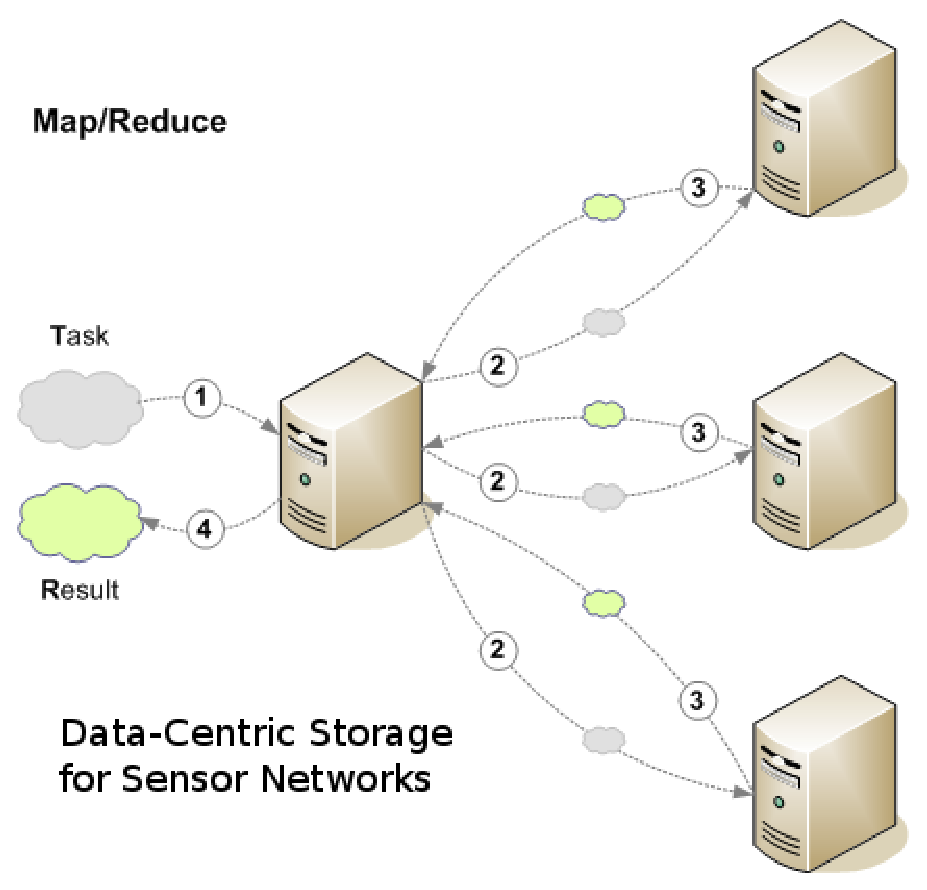
\includegraphics[scale=0.5]{../diagrams/future-works-data-centric-map-reduce}
  \caption{Data-Centric approach using MapReduce to search accross different
  database shards}
  \label{fig:future-works-data-centric-map-reduce}
\end{figure}

In addition to infrastructural, the use techniques for scheduling data
gathering from the SF-BEAMS sensor networks can be used to decrease the data
load into the system. While the period of times used by the RTC seems
to cover the basic requirements of data, the data storage may be
seen as overloaded with repeated data. Since environmental conditions
does not change drastically over time, the use of data scheduling and
data clustering approaches can be used. First, considering that SF-BEAMS
contains a cluster of sensors, the data load could be decreased by using
techniques such as clustering the data in the data sink before they are
persisted \cite{sn-time-series, sn-schedule-minimal-aggregation-time}. Since
the infrastructure of the SF-BEAMS sensor network is a one-hop start design,
the knowledge about the data can only be achieved in the data sink. In this
way, one suggestion is the implementation of a DSP Data Clustering component
that is responsible for the data clustering before they are inserted into the
database. Similarly, the use of schedulers on the sensors could also be used to
decrease the amount of data to be sent to the data sink, as seen at the survey
\cite{sn-scheduling-survey}. 

Finally, taking into account the use of the database system to complement
NetBEAMS execution, the design of event-based applications could add different
functionalities to the management capabilities of the sensor networks. For
instance, the YSI sonde collected data carries the information regarding the
battery life of the device, seen at the collected attribute 
``observation.Battery''. A new DSP Component responsible for observing these
attributes could define the threshold of the event of low-battery. With an
event-based application in mind, events regarding the SF-BEAMS network could be
better managed through NetBEAMS where scheduled sites visits would depend on
such events to happen and, thus, avoiding unecessary operational costs.